\documentclass{beamer}

\mode<presentation>
{
  \usetheme{Warsaw}
  \setbeamercovered{transparent}
}
\usepackage[english]{babel}
\usepackage[utf8]{inputenc}
\usepackage{times}
\usepackage{float}
\usepackage[T1]{fontenc}

\title[PROYECTO - PYTHON] 
{M A Z E S}


\subtitle{}
\institute[ESCUELA SUPERIOR]
{	
	\centering
  		%
\includegraphics[totalheight=1in,width=1in]{ss}
  		
	ESCUELA SUPERIOR\\
	POLITECNICA DEL LITORAL
}
\date[CFP 2013]{Proyecto en Python, 2013}

\begin{document}
	\begin{frame}
  	  \titlepage
	\end{frame}
	
	%Integrantes del Grupo
	\begin {frame}{INTEGRANTES}
		 \begin{flushleft}
 			
\includegraphics[totalheight=1.2in,width=2in]{LTwitspol}
 		 \end{flushleft}
 		 
 		 \begin{itemize}
 		 	\item
				\begin{flushright} 		 		
 		 		Torres Criollo Daniel
 		 		\end{flushright}
 		 	\item
 		 		\begin{flushright}
 		 			Velez Gomez José
 		 		\end{flushright}
 		 \end{itemize}
  	\end{frame}
  	  	
  	%Seccion Introduccion
  	\begin{frame}{DESCRIPCION DEL JUEGO}
  		\centering
  		 %
\includegraphics[totalheight=1in,width=1in]{ss}
  		\begin{block}{}
  		El juego comienza siempre desde el nivel 1, donde en un cierto punto el jugador tendra que elegir por donde ir de 2 opciones y si la pasa satisfactoriamente, llegara al otro extremo y pasara al siguiente nivel que es el NIVEL 2 que tambine tiene varios caminos para llegar al otro extremo pero tambien tiene obstaculo que unos de ellos puede ser que termine el juego y pierda, pero si paso al otro extremo pasare al siguiente nivel que es el NIVEL 3 que al pasar al otro extremo terminara el juego.
  		\end{block}				
	\end{frame}
	
	\begin{frame}{FUNCIONALIDADES DEL JUEGO}
		\centering
  		%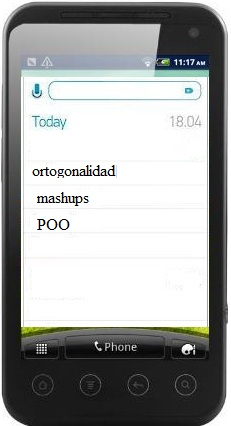
\includegraphics[totalheight=1.4in,width=0.9in]{lt}
  		\begin{block}{}
  		En este juego elaborado en Python, tratamos de hacerlo en funcion que tambien utilicemos sonidos creado por nosotros mismo, para de cierta forma guiarnos de cual decision tomar, no sabiendo aun con que obstaculo nos encontraremos y en transcurso del camino del laberinto;REGRESAR al inicio o PERDER el juego.	
  		\end{block}				
	\end{frame}
	
  	

\begin{frame}{OBSERVACIONES}
		\centering
  		\begin{block}{}
  		Desarrollar en Python por primera vez requiere de mucha paciencia, tener conocimiento en programacion.
		\end{block}
		
  		\begin{block}{}
		Tener mucho cuidado con las colisiones.
  		\end{block}
		
 	\end{frame}


\begin{frame}{EXPERIENCIAS}
		
\includegraphics[width=0.3\textwidth]{pygame}
		\centering
  		\begin{block}{}
  		Adquirimos algo de experiencia, ya que era nuestra primera incursión en el desarrollo en Phyton y Pygame.
  		\end{block}
		\begin{block}{}
		Tuvimos inconvenientes con el IDE y demás cuestiones de instalación.
  		\end{block}
		\begin{block}{}
		Fué de gran ayuda el uso de internet, ya que hay muchos soportes, foros, tutoriale, etc.
  		\end{block}
 	\end{frame}

\begin{frame}{CONCLUSIONES}
		\centering
  		\begin{block}{}
		Lo interesante de programar en un lenguaje nuevo para nosotros, significo reto nuevo.
  		\end{block}
  		\begin{block}{}
		El hecho de implementar las funcionalidades no fue muy complejo.
  		\end{block}
  		\begin{block}{}
		La funcionalidad de nuestra aplicación no era trivial.
  		\end{block}
  		
 	\end{frame}


		
	%\appendix	
	%\section<presentation>*{\appendixname}
	\subsection<presentation>*{DIFICULTADES-LABERINTOS -- PYTHON}
	\begin{frame}
	\centering
	
\includegraphics[width=0.3\textwidth]{python}
		
		\begin{center}
			M U C H A S \\ G R A C I A S 
		\end{center}
	\end{frame}
	
	
\end{document}

